\documentclass[a4paper,titlepage]{article}
\usepackage{lingmacros}
\usepackage{tree-dvips}
\usepackage[italian]{babel}
\usepackage[utf8x]{inputenc}
\usepackage{amssymb}
\usepackage{graphicx}
%\usepackage{frontespizio}

\begin{document}
\tableofcontents

\newpage
\section{Introduzione}
In questo documento verranno presentati gli argomenti trattati per lo svolgimento del progetto di Sistemi con Vincoli, realizzato dagli studenti Rango Massimiliano, Segato Silvia e Tesselli Riccardo.\\Il progetto di interesse riguarda lo sviluppo di un risolutore automatico di CP-Nets sia acicliche che cicliche che adotta varie strategie di risoluzione.\\In questo documento verrà prima introdotto il problema iniziale, successivamente verranno presentate le fasi di lavoro svolte e descritte le nostre soluzioni al problema. Saranno poi visualizzati e analizzati i risultati ottenuti e infine presentato il consuntivo delle ore di lavoro e le istruzioni d'uso del software realizzato.

\section{Presentazione del Problema}
Una CP-Net è una struttura che rappresenta reti di preferenze condizionali. Più formalmente una CP-Net sulle variabili $V = \{X_{1},\dots, X_{n}\}$ è un grafo orientato sui nodi $X_{1},\dots, X_{n}$, ogni nodo $X_{i} \in V$ è annotato con una tabella di preferenze condizionali $CPT(X_{i})$. Ogni tabella di preferenze condizionali $CPT(X_{i})$ associa un ordine totale $\succ^{i}_{\textbf{u}}$ con ogni instanziazione \textbf{u} dei genitori di $X_{i}$ detti $Pa(X_{i}) = U$. Una CP-Net si dice aciclica se il grafo che rappresenta non contiene cicli, altrimenti è detta ciclica.\\
Nel problema dato si vogliono individuare le soluzioni ottime, se esistono, di una CP-Net aciclica o ciclica, e individuare l'ordinamento parziale delle sue soluzioni. La ricerca delle soluzioni ottime è stata affrontata con diversi approcci. Il linguaggio di programmazione adottato è Java.\\Nella sessione successiva verranno presentate le varie fasi di lavoro.


\section{Fasi di Sviluppo}

\subsection{Generazione Casuale di CPNets}
In primo luogo è stato sviluppato un codice per la generazione di CP-Nets casuali a partire da alcuni parametri scelti dall'utente, al fine di poter studiare il comportamento delle varie strategie di risoluzione al variare della struttura della CP-Net.\\
Il software genera una CP-Net in maniera casuale con numero di nodi e numero di archi fissati dall'utente. Per ogni nodo si generano le preferenze casualmente, supponendo che ogni nodo possa assumere due valori (negato o affermato), le preferenze generate garantiscono che il numero di condizioni per cui si preferisce il valore negato corrisponda al numero di condizioni per cui si preferisce il valore affermato, ovvero siano equamente distribuite.\\
Per la creazione l'algoritmo in primo luogo genera un grafo con il numero di nodi fissato dall'utente, ad ogni nodo viene assegnato un nome che corrisponde al numero cardinale del momento di creazione; successivamente estrae casualmente due nodi del grafo, uno di inizio e uno di fine, se dal nodo di inizio al nodo di fine non esiste già un arco orientato tra essi allora ne inserisce uno. Si continua a inserire archi fintanto che il numero di archi non corrisponde al parametro inserito dall'utente.\\
Come si può notare l'algoritmo di creazione di CP-Nets casuali può generare indistintamente reti cicliche o acicliche. Per distinguere la ciclicità di una CP-Net è stato sviluppato un algoritmo che controlla l'esistenza di cicli in un grafo orientato.
\subsection{Strategie di Base}
I primi algoritmi implementati per trovare le soluzioni ottime di CP-Nets sono quelli appresi e messi in pratica a lezione.

\subsubsection{Algoritmo per CP-Nets acicliche: Sweep Forward}
L'algoritmo implementato per trovare l'unica soluzione ottima di una CP-Net aciclica è denominato Sweep Forward e consiste nel seguire le dipendenze del grafo. In particolare, consiste nell'assegnare il valore ``preferito'' ad ogni variabile nel contesto degli assegnamenti fatti per i genitori.

\subsubsection{Algoritmo per CP-Nets cicliche}
Data una CP-Net ciclica, per trovare le sue soluzioni ottime si deve ricavare un insieme di vincoli $P$, tale che le soluzioni di $P$ coincidono con l'insieme delle soluzioni ottime della CP-Net. Tale insieme $P$ lo si riesce a  trovare in tempo polinomiale.

\subsubsection{Implementazione}
Il metodo che si occupa di trovare le soluzioni ottime della CP-Net generata è il seguente
\\
\\
\centerline{\texttt{public List<Assignment> getOptimalSolution(Inference strategy, boolean findAll)}}
\\

Tale metodo adotta le due strategie descritte sopra in base alla ciclicità della CP-Net data.
Ogni soluzione ottima della CP-Net è stata implementata come assegnamento (oggetto di tipo \texttt{Assignment}); un assegnamento è una mappa $\langle$variabile, valore$\rangle$.
L'algoritmo Sweep Forward per CP-Nets acicliche è stato implementato come metodo della classe \texttt{CPNet}:\\
\\
\centerline{\texttt{public Assignment solveAcyclicCPNet(Assignment result, List<Variable> vars)}}
\\

La soluzione ottima in questo caso corrisponde alla variabile \texttt{result}.
Per ciascuna variabile indipendente, viene settato in \texttt{result} il relativo assegnamento con il valore preferito.
Dopo ciò si controllano le variabili non indipendenti, precedentemente inserite in una lista; per ciascuna di queste, si controlla se i suoi genitori hanno già un valore assegnato in \texttt{result}. Se così è, allora in base all'assegnamento dei genitori si sceglie il valore preferito per la variabile in esame e lo si usa per settare l'assegnamento di quest'ultima in \texttt{result}. Fatto ciò si toglie la variabile dalla lista e si ricomincia l'analisi con le rimanenti variabili. Qualora la variabile in esame non avesse ancora una configurazione completa per tutti i suoi genitori, la si lascia nella lista e si prosegue con la successiva.
\\
Al fine di poter attuare la strategia di risoluzione per CP-Nets cicliche, il primo passo da effettuare è la conversione da CP-Net a CSP. 
\\
I CSPs che si vengono a creare consistono di variabili, ciascuna delle quali ha come dominio \{0, 1\}, e un insieme di vincoli.
A livello implementativo, ciò corrisponde alla creazione della classe \texttt{CSP} e \texttt{Variable}, nonché dell'interfaccia \texttt{Constraint}.
 
I vincoli rispettano il seguente pattern:
\\
\centerline{ipotesi $\rightarrow$ tesi}

Tesi e ipotesi si compongono di assegnamenti. La tesi contiene l'assegnamento di un unica variabile, l'ipotesi contiene disgiunzioni di congiunzioni di assegnamenti (ad esempio, la seguente può essere una ipotesi: $( (A=1 \land B=1) \lor (A=0 \land B=0))$ ). 

Tale tipo di vincolo è stato implementato con la creazione della classe \texttt{Implies}, che implementa \texttt{Constraint}.


La classe \texttt{CPNetCSP} si occupa di creare un CSP di questo tipo, dopo aver opportunamente creato le variabili a partire dai vertici del grafo, tramite il metodo
\\
\centerline{\texttt{private List<Variable> generateVariables()}}
\\
e i vincoli a partire dalle preferenze,tramite il metodo
\\
\centerline{\texttt{private List<Implies> generateConstraints(List<Variable> variables)}}
\\

Per trovare le soluzioni del CSP così creato è stata utilizzata la classe astratta\texttt{SolvingStrategy} e la sua sottoclasse \texttt{BacktrakingStrategy}. Come dice il nome stesso, tale classe si occupa di implementare la strategia di risoluzione di un CSP attraverso la ricerca con Backtraking. L'algoritmo implementato è in grado di trovare tutte le soluzioni ottime del CSP datogli in input. Tuttavia, l'utente finale può scegliere se lasciare che l'algoritmo trovi tutte le soluzioni o si fermi alla prima soluzione.

L'utente è anche in grado di scegliere se eseguire l'algoritmo di Backtraking ``di base'', o se con Forward Checking o con propagazione di vincoli (AC3). Per permettere ciò, si è utilizzata una sottoclasse di \texttt{BacktrakingStrategy}, denominata \texttt{ImprovedBacktrakingStrategy}, e una nuova classe, \texttt{AC3Strategy}, che si occupa della propagazione di vincoli.



\subsection{Ordinamento Parziale delle Soluzioni}

Per poter ottenere l'ordinamento parziale delle soluzioni, occorre eseguire il metodo
\\
\centerline{\texttt{public boolean generatePartialOrderSolution()}}
\\

Tale metodo si occupa di creare un oggetto \texttt{PartialOrderSolutionGraph}, che rappresenta il grafo delle soluzioni. In particolare,  l'oggetto contiene una lista di oggetti \texttt{Solution}, ognuno dei quali contiene, oltre al valore della soluzione stessa che, per brevità, è una stringa (ad esempio, in una CP-Net che ha, nell'ordine, A, B, C come variabili, un oggetto \texttt{Solution} ha come valore ``111'', che è da intendersi come l'equivalente di {A=1, B=1, C=1}), anche la lista dei valori di quelle soluzioni che sono sotto di lei nell'ordinamento (da ora in avanti queste verranno chiamate ``sottoliste'').
Per costruire il grafo vero e proprio, viene richiamato il metodo 
\\
\centerline{\texttt{public void setPartialOrderSolutions()}}
\\

Esso si occupa di settare le sottoliste di ciascuna 
soluzione. In questo modo, il grafo viene memorizzato come una lista di adiacenze.

\subsection{Strategia con Local Search}
Come approccio alternativo alle strategie di risoluzione viste in precedenza è stata realizzata la ricerca delle soluzioni ottime di una CP-Net tramite un approccio di ricerca locale. Lo sviluppo di una tecnica Local Search è stata di nostro interesse in quanto tale strategia si adatta molto bene allo spazio di ricerca delle soluzioni. In primo luogo perché in tale spazio si ha un chiaro concetto di ``vicinanza'' tra due soluzioni; in secondo luogo poiché la struttura dello spazio di ricerca fa si che l'ottimo locale tipicamente sia l'ottimo globale, a meno di plateaux. Infatti nel caso di CP-Nets acicliche sappiamo che esiste una sola soluzione ottima, e un algoritmo di ricerca locale convergerà ad esso, in quanto ad ogni step migliorativo ci avviciniamo sempre più alla assegnazione ottima. Nel caso di CP-Nets cicliche possiamo avere casi non così chiari, nel caso specifico quando non esiste una sola soluzione ottima, ma esistono varie soluzioni parimenti preferibili sebbene non ottime in assoluto. In questo caso l'approccio Local Search non potrà mai convergere ad una soluzione più preferibile di altre.
\subsubsection{Implementazione}
Il metodo dell'oggetto \texttt{CPNet} che realizza tale strategia è \texttt{solveWithLocalSearch}. Tale metodo implementa una tecnica Hill Climbing. Per descrivere meglio come opera l'algoritmo è preferibile introdurre dei concetti sullo spazio di ricerca. Lo spazio di ricerca sul quale opera l'algoritmo Local Search è rappresentato da un grafo orientato, i cui nodi rappresentano le possibili assegnazioni delle variabili. Tra due assegnazioni vicine, ossia tra due assegnazioni che differiscono solo per un assegnamento diverso per una sola variabile esiste un arco orientato. Se l'assegnazione $A$ è migliore della assegnazione $B$ allora esiste un arco diretto da $A$ a $B$. In questo contesto quindi la soluzione ottima per definizione è quella che non ha vicini migliori di essa, ossia la soluzione con soli archi uscenti. Viceversa la soluzione pessima è rappresentata dal nodo con soli archi entranti, in quanto ogni vicino è migliore di essa. Se tra due nodi $A$ e $B$ non esiste un cammino orientato significa che le due soluzioni non sono confrontabili.\\
Ora che è stata introdotta la terminologia possiamo presentare il funzionamento dell'algoritmo. In primo luogo viene generata una assegnazione casuale delle variabili, essa quindi rappresenta il nodo di partenza all'interno del grafo delle soluzioni. Sia $A$ il nodo correntemente visitato dall'algoritmo di ricerca, ad ogni passo di ricerca vengono esaminati i suoi vicini in ordine casuale. Non appena viene individuato un vicino $B$ migliore di $A$ (ossia se esiste un arco diretto da $B$ ad $A$) allora l'algoritmo si sposta verso $B$, graficamente ciò equivale a percorrere il grafo seguendo il verso contrario delle frecce. La determinazione di nodo migliore o peggiore è determinata osservando la tabella di preferenza condizionale della variabile per cui le due assegnazioni differiscono. Se un nodo non ha vicini migliori significa che è l'ottimo. La ricerca prosegue fintanto che non viene individuata una soluzione ottima o non viene raggiunto il limite massimo di iterazioni fissato. Empiricamente è stato osservato che un limite di iterazioni massimo fissato a 10000 è molto più che sufficiente anche su grafi molto complessi.


\section{Risultati e Statistiche}
In questa sezione vengono descritti i test effettuati sul sistema e presentati i risultati ottenuti. I test intendono mostrare il tempo di risoluzione medio delle varie strategie implementate al variare della dimensione della CP-Net. Di seguito vengono prima presentati i test effettuati su CP-Net acicliche e successivamente su quelle cicliche; successivamente verranno mostrati alcuni risultati sul comportamento della strategia Local Search.
\subsection{Test su CP-Net Acicliche}
Per la risoluzione di CP-Net acicliche sono state implementate le strategie Sweep Forward e Local Search. Il primo test svolto mostra come varia il tempo di risoluzione medio delle due strategie al crescere del numero di archi, con numero di nodi fissato. Le medie si basano su 10 prove. Nelle Figure \ref{fig:test1}, \ref{fig:test2}, \ref{fig:test3} vengono visualizzati i risultati ottenuti variando il numero di archi su una CP-Net con rispettivamente 10, 30 e 50 nodi. La precisione di misura è al millesimo di secondo.
\begin{figure}[!h]
\centering
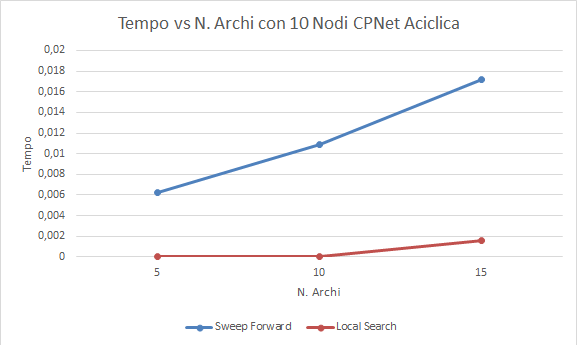
\includegraphics[scale=0.8]{../img/10NodiAciclica.png}
\caption{Tempo di risoluzione (s) al crescere del numero di archi su CP-Net aciclica con 10 nodi}\label{fig:test1}
\end{figure}
\begin{figure}[!h]
\centering
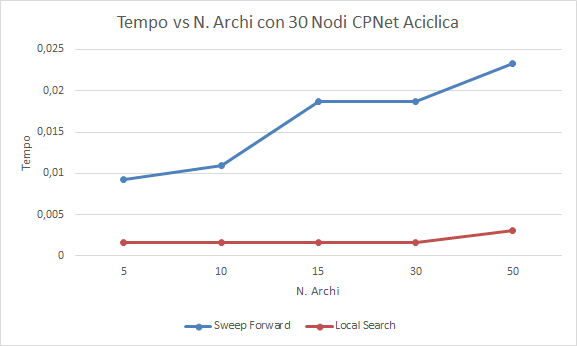
\includegraphics[scale=0.8]{../img/30NodiAciclica.png}
\caption{Tempo di risoluzione (s) al crescere del numero di archi su CP-Net aciclica con 30 nodi}\label{fig:test2}
\end{figure}
\begin{figure}[!h]
\centering
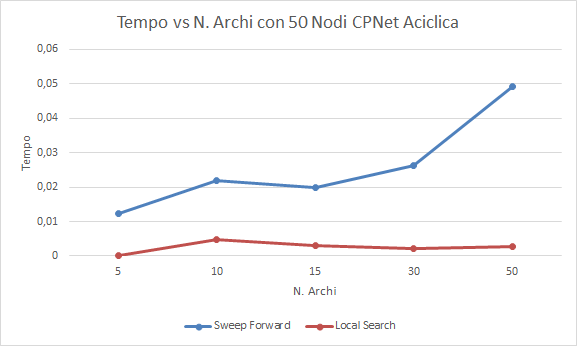
\includegraphics[scale=0.8]{../img/50NodiAciclica.png}
\caption{Tempo di risoluzione (s) al crescere del numero di archi su CP-Net aciclica con 50 nodi}\label{fig:test3}
\end{figure}
\\\'E possibile osservare i diversi comportamenti delle due strategie. Sweep Forward cresce linearmente al crescere del numero di archi, mentre Local Search sembra essere pressoché costante, sebbene vi sia un lieve aumento nel tempo di risoluzione. Sotto queste condizioni l'approccio Local Search dà buoni risultati, in quanto è meno sensibile all'aumento di dimensione della CP-Net e garantisce di individuare l'ottimo globale in un numero modesto di iterazioni.\\
Per completezza in Figura \ref{fig:test8} vengono mostrati i risultati al variare del numero di nodi fissando il numero di archi.
\begin{figure}[!h]
\centering
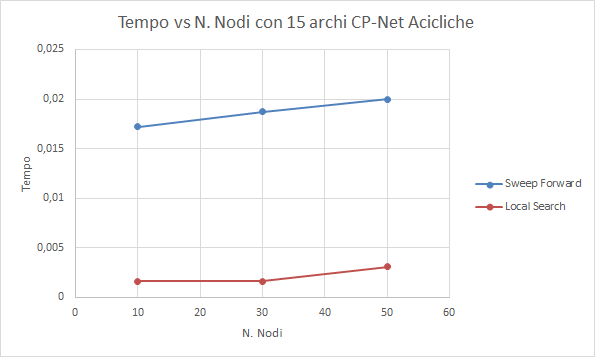
\includegraphics[scale=0.8]{../img/15ArchiAciclica.png}
\caption{Tempo di risoluzione (s) al crescere del numero di nodi su CP-Net aciclica con 15 archi}\label{fig:test8}
\end{figure}
\\\'E possibile osservare un comportamento analogo a quello precedentemente descritto.
\subsection{Test su CP-Net Cicliche}
Per la risoluzione di CP-Net cicliche sono state realizzate le seguenti strategie: ricerca con Backtracking, Backtracking con Forward Checking, Backtracking con propagazione vincoli d'arco e Local Search.\\
Il test effettuato intende mostrare il tempo di risoluzione medio al crescere del numero di archi di una CP-Net dato un numero di nodi fissato. Le medie si basano su 10 prove. Nelle Figure \ref{fig:test4}, \ref{fig:test5}, \ref{fig:test6} vengono visualizzati i risultati ottenuti variando il numero di archi su una CP-Net con rispettivamente 10, 30 e 50 nodi. La precisione di misura è al millesimo di secondo.
\begin{figure}[!h]
\centering
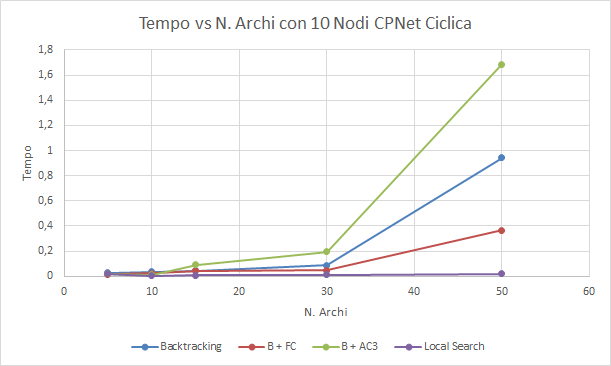
\includegraphics[scale=0.75]{../img/10NodiCicliche.png}
\caption{Tempo di risoluzione (s) al crescere del numero di archi su CP-Net ciclica con 50 nodi}\label{fig:test4}
\end{figure}
\begin{figure}[!h]
\centering
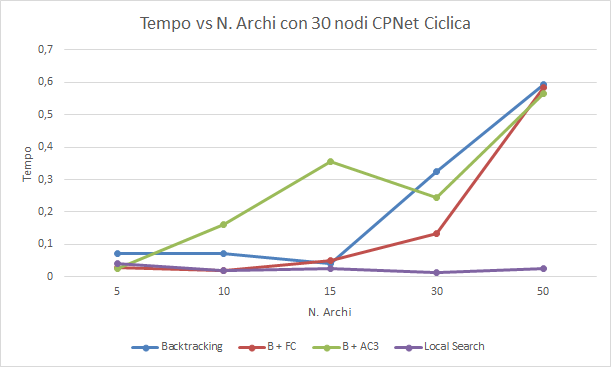
\includegraphics[scale=0.75]{../img/30NodiCicliche.png}
\caption{Tempo di risoluzione (s) al crescere del numero di archi su CP-Net ciclica con 50 nodi}\label{fig:test5}
\end{figure}
\begin{figure}[!h]
\centering
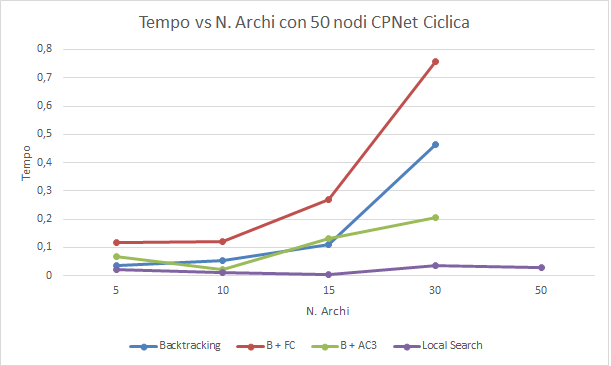
\includegraphics[scale=0.75]{../img/50NodiCicliche.png}
\caption{Tempo di risoluzione (s) al crescere del numero di archi su CP-Net ciclica con 50 nodi}\label{fig:test6}
\end{figure}
\\Nel caso di CP-Net cicliche osserviamo dai dati una crescita di tempo esponenziale all'aumentare del numero di archi. In particolar modo questo è evidente in Figura \ref{fig:test6} dove non è stato possibile effettuare i test per 50 archi in quanto il tempo di esecuzione era al di fuori della nostra portata. Si nota inoltre come l'approccio Local Search mantenga gli stessi standard che abbiamo visto in precedenza, sebbene in questo caso ci sia da fare una precisazione. I dati raccolti per la strategia Local Search nel caso di CP-Net cicliche si riferiscono esclusivamente ai casi in cui la CP-Net abbia almeno una soluzione globalmente ottima. Nel caso ciò non si verificasse l'algoritmo Local Search non è in grado di individuare la soluzione globalmente ottima, saturando quindi il numero di iterazioni massime consentito.\\
Alla luce di ciò notiamo come Local Search sia ancora una valida strategia per l'individuazione della soluzione ottima, ma purtroppo, nella maggior parte dei casi di CP-Net cicliche, ciò non accade, e bisogna ricorrere alle strategie convenzionali, sebbene il tempo di esecuzione cresca esponenzialmente. Per argomentare ulteriormente questa tesi viene presentata in Figura \ref{fig:test7} l'aumento esponenziale del tempo all'aumentare della complessità della CP-Net. Sono state considerate CP-Net che rappresentano grafi completi K5, K7 e K10.
\begin{figure}[!h]
\centering
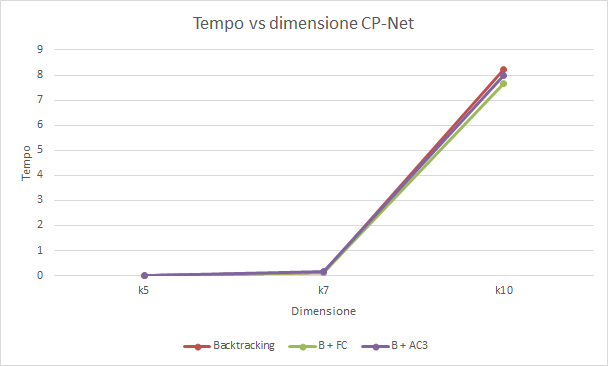
\includegraphics[scale=0.75]{../img/TempoK.png}
\caption{Tempo di risoluzione (s) su grafi completi}\label{fig:test7}
\end{figure}
\\Si può facilmente notare la crescita esponenziale di queste strategie al crescere della complessità.
\subsection{Test su Local Search}
Sono stati effettuati test più specifici per la strategia Local Search al fine di studiare come varia il numero di iterazioni per la ricerca della soluzione ottima al variare della struttura della CP-Net.\\
In Figura \ref{fig:test9} viene mostrato il numero di iterazioni effettuate per individuare la soluzione ottima al crescere del numero di archi per tre serie di CP-Net acicliche da 10, 30 e 50 nodi.
\begin{figure}[!h]
\centering
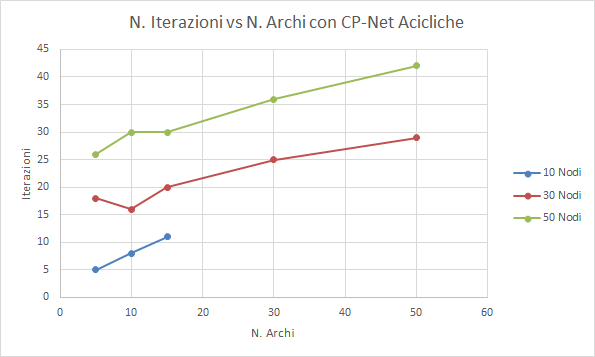
\includegraphics[scale=0.75]{../img/IterazioniAciclica.png}
\caption{Numero iterazioni di ricerca locale al crescere del numero di archi su CP-Nets acicliche}\label{fig:test9}
\end{figure}
\\Per la serie da 10 nodi non è stato possibile ottenere dati per numero di archi oltre 15 in quanto era difficoltoso ottenere grafi aciclici con tali parametri.\\
Analogamente in Figura \ref{fig:test10} vengono mostrate le stesse statistiche descritte in precedenza su CP-Net cicliche.
\begin{figure}[!h]
\centering
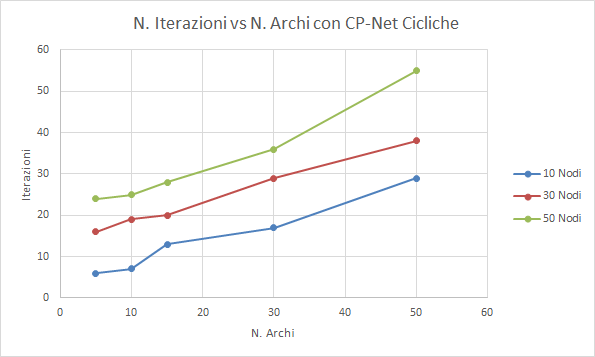
\includegraphics[scale=0.75]{../img/IterazioniCicliche.png}
\caption{Numero iterazioni di ricerca locale al crescere del numero di archi su CP-Nets cicliche}\label{fig:test10}
\end{figure}
\\Si osserva una correlazione lineare tra il numero di iterazioni e il numero di archi, inoltre si osserva che all'aumentare del numero dei nodi i risultati ottenuti variano per una costante, sia nel caso di CP-Net acicliche che cicliche.
\subsection{Conclusioni}
Dai risultati ottenuti si può affermare che per CP-Nets acicliche la strategia Local Search si rivela estremamente efficace. Tale efficacia si riscontra anche nel caso di CP-Nets cicliche che presentano almeno una soluzione globalmente ottima. Nel caso peggiore tale strategia è inutile e quindi è necessario ricorrere alle strategie con ricerca tradizionale. Tali strategie sono esponenzialmente correlate alla complessità della CP-Net, inoltre la presenza di strategie di supporto alla ricerca con Backtracking (Forward Checking e propagazione dei vincoli d'arco) sembrano non influire eccessivamente sui tempi di esecuzione.
\section{Consultivo Finale}
In questa sezione viene presentato il consuntivo delle ore di lavoro effettuate. Il carico di lavoro è stato equamente diviso tra i tre membri sui vari aspetti del progetto, pertanto viene presentato il carico di ore medio per un membro del gruppo.
\begin{itemize}
\item Documentazione e ricerca dei materiali di lavoro: 2 ore;
\item Implementazione generazione casuale CP-Net: 2 ore;
\item Sviluppo front-end di visualizzazione: 1 ora;
\item Implementazione strategie di base: 4 ore;
\item Realizzazione ordinamento parziale delle soluzioni: 4 ore;
\item Implementazione strategie Local Search: 3 ore;
\item Test e debug: 3 ore;
\item Raccolta statistiche: 3 ore;
\item Stesura relazione: 2 ore;
\item Realizzazione presentazione: 1 ora;
\item \textbf{Totale}: 25 ore a persona.
\end{itemize}


\section{Appendice: Istruzioni d'Uso}
Il software viene fornito sotto forma di JAR eseguibile. Per lanciare l'esecuzione bisogna eseguire da console il comando
\begin{verbatim}
java -jar CPNets.jar <strategy> <nNodi> <nArchi> <findAll>
\end{verbatim}
dove \texttt{<strategy>}, \texttt{<nNodi>}, \texttt{<nArchi>}, \texttt{<findAll>} sono i parametri.\\
Il parametro \texttt{<strategy>} definisce con quale strategia si vogliono individuare le soluzioni della CP-Net, i valori ammessi sono:
\begin{itemize}
\item  \texttt{ls} : Local Search;
\item  \texttt{fc} : Backtracking + Forward Checking;
\item  \texttt{ac3} : Backtracking + consistenza d'arco;
\item  \texttt{none} : Backtracking.
\end{itemize}
I parametri \texttt{<nNodi>}, \texttt{<nArchi>} definiscono rispettivamente il numero di nodi e archi della CP-Net da generare.\\
Infine il parametro \texttt{<findAll>} è un parametro booleano, se è \texttt{true} allora l'algoritmo di risoluzione individuerà tutte le soluzioni ottime del problema, se altrimenti è \texttt{false} verrà individuata solo la prima ottima individuata. Questo parametro viene utilizzato solo nel caso di strategie che richiedono Backtracking, non si applica alla strategia Local Search.\\
Una volta lanciato il comando comparirà una interfaccia grafica come visualizzato in Figura \ref{fig:1}.\\
\begin{figure}
\centering
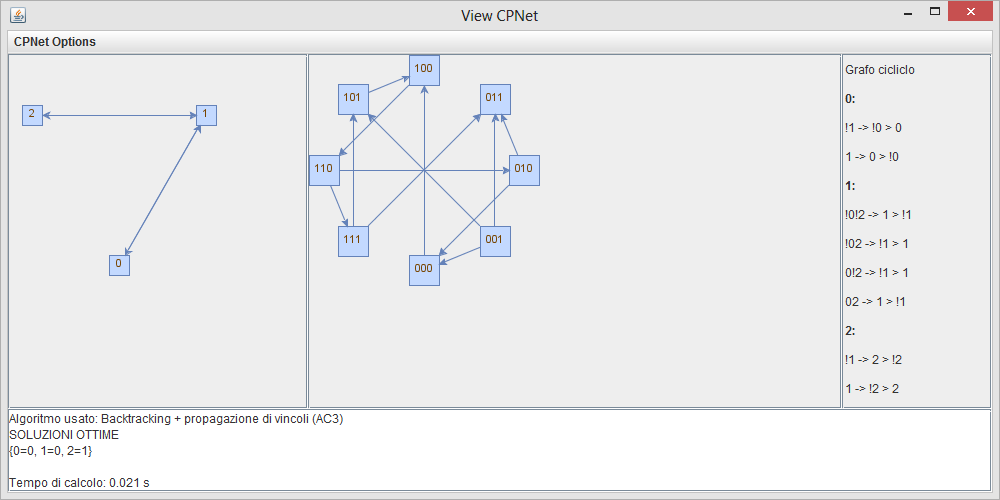
\includegraphics[scale=0.5]{../img/screen.png}
\caption{Esempio di schermata}\label{fig:1}
\end{figure}
Nel riquadro a sinistra viene visualizzata la struttura della CP-Net; nel pannello a destra viene mostrata la ciclicità della rete e le tabelle di preferenze condizionali di ogni variabile. Si assume che data una variabile $X$ i valori per tale variabile sono $x$ per i valori affermati e $!x$ per i valori negati.\\
Nel pannello centrale viene visualizzato il grafo che rappresenta l'ordinamento parziale di tutte le soluzioni della CP-Net. Ogni nodo del grafo rappresenta una instanziazione dei valori delle variabili. Una instaziazione è intesa come un assegnamento ordinato di valori 0, per valori negati, e 1 per valori affermati. L'ordine di assegnazione è determinato in senso crescente, ovvero il primo valore si riferisce alla variabile 0 e così via fino all'ultima variabile. Se una instanziazione $A$ è migliore di una instanziazione $B$ allora compare un arco orientato da $A$ a $B$ nel grafo. Per visualizzare l'ordinamento parziale delle soluzioni è necessario cliccare sul menù a tendina in alto a sinistra.\\
Nel pannello inferiore viene visualizzato un riassunto della strategia utilizzata, della soluzione ottima individuata e del tempo di calcolo richiesto.

\end{document}